% !TeX program = xelatex
\documentclass[a4paper,10pt]{article}

% ============================================================================
% កញ្ចប់បណ្ណាល័យ (Packages) – តាមលំនាំស្តង់ដារ អនុវិទ្យាល័យព្រះក្រសាំង (ls_plan.tex)
% បរិបទ៖ ថ្នាក់រៀនគ្មានស្លាយ LCD – បង្រៀនដោយប្រើក្ដារខៀន បន្ទាត់ក្រិត ដែកឈាន និងសន្លឹកកិច្ចការស-ខ្មៅ
% ============================================================================
\usepackage[a4paper, left=0.95cm, right=0.95cm, top=0.85cm, bottom=0.92cm, footskip=0.52cm]{geometry}
\usepackage{amsmath}
\usepackage{unicode-math}
\usepackage{fontspec}
\usepackage{array, longtable, multirow, colortbl}
\usepackage[table]{xcolor}
\usepackage{enumitem}
\usepackage{pifont}
\usepackage{fancyhdr}
\usepackage{tikz}
\usetikzlibrary{calc, arrows.meta, angles, quotes, decorations.markings, positioning, babel}

\makeatletter
\let\@expl@@@mark@update@singlecol@structures@@\relax
\makeatother

% ============================================================================
% ការកំណត់ពុម្ពអក្សរផ្លូវការ (Cross-Platform Fonts Configuration)
% ============================================================================
\providecommand{\NGSFindFonts}{%
  \IfFileExists{C:/Windows/Fonts/cambria.ttc}{%
    \def\NGSSysPath{C:/Windows/Fonts/}%
    \def\NGSUserPath{C:/Users/KIT/AppData/Local/Microsoft/Windows/Fonts/}%
  }{%
    \IfFileExists{./fonts/KhmerOSsiemreap.ttf}{\def\NGSSysPath{./fonts/}\def\NGSUserPath{./fonts/}}{%
    \IfFileExists{../fonts/KhmerOSsiemreap.ttf}{\def\NGSSysPath{../fonts/}\def\NGSUserPath{../fonts/}}{%
    \IfFileExists{../../fonts/KhmerOSsiemreap.ttf}{\def\NGSSysPath{../../fonts/}\def\NGSUserPath{../../fonts/}}{%
    \IfFileExists{../../../fonts/KhmerOSsiemreap.ttf}{\def\NGSSysPath{../../../fonts/}\def\NGSUserPath{../../../fonts/}}{%
    \IfFileExists{../../../../fonts/KhmerOSsiemreap.ttf}{\def\NGSSysPath{../../../../fonts/}\def\NGSUserPath{../../../../fonts/}}{%
    \IfFileExists{../../../../../fonts/KhmerOSsiemreap.ttf}{\def\NGSSysPath{../../../../../fonts/}\def\NGSUserPath{../../../../../fonts/}}{%
    \IfFileExists{../../../../../../fonts/KhmerOSsiemreap.ttf}{\def\NGSSysPath{../../../../../../fonts/}\def\NGSUserPath{../../../../../../fonts/}}{%
      \def\NGSSysPath{../../../../../../../fonts/}\def\NGSUserPath{../../../../../../../fonts/}%
    }}}}}}}%
  }%
}
\NGSFindFonts

\setmathfont[Path={\NGSSysPath}, FontIndex=1, Scale=1.02]{cambria.ttc}
\defaultfontfeatures{Ligatures=TeX}

\setmainfont[
  Path={\NGSUserPath},
  Extension=.ttf,
  Script=Khmer,
  BoldFont={KhmerOSsiemreap},
  BoldFeatures={FakeBold=1.8},
  ItalicFont={KhmerOSsiemreap},
  ItalicFeatures={FakeSlant=0.25},
  BoldItalicFont={KhmerOSsiemreap},
  BoldItalicFeatures={FakeBold=1.8, FakeSlant=0.25}
]{KhmerOSsiemreap}

\newfontfamily\muol[Path={\NGSUserPath}, Extension=.ttf, Script=Khmer]{KhmerOSmuollight}
\newfontfamily\TimesEn[Path={\NGSSysPath}, Extension=.ttf, BoldFont={timesbd}, ItalicFont={timesi}, BoldItalicFont={timesbi}]{times}
\newfontfamily\NagaBold[Path={\NGSUserPath}, Extension=.ttf]{AKbalthom Naga Bold}
\newfontfamily\CalibriFont[Path={\NGSSysPath}, Extension=.ttf]{calibri}
\newfontfamily\Tacteing[Path={\NGSUserPath}]{TACTENG.TTF}
\newfontfamily\CourierBullet[Path={\NGSSysPath}, Extension=.ttf]{cour}
\newcommand{\wcirc}{{\CourierBullet\fontsize{9.5pt}{11pt}\selectfont o}}

\XeTeXlinebreaklocale "km"
\XeTeXlinebreakskip = 0pt plus 1pt minus 0.1pt

\definecolor{stepgray}{HTML}{D9D9D9}
\definecolor{headgray}{HTML}{F2F2F2}
\definecolor{boxgray}{HTML}{D9D9D9}
\definecolor{darkred}{HTML}{C00000}
\definecolor{red5e}{HTML}{FF0000}

\pagestyle{fancy}
\fancyhf{}
\renewcommand{\headrulewidth}{0pt}
\fancyfoot[R]{\CalibriFont\fontsize{11pt}{13pt}\selectfont\thepage}

\setlength{\parindent}{0pt}
\setlength{\parskip}{0pt}
\setlength{\tabcolsep}{3.8pt}

\newcolumntype{L}[1]{>{\raggedright\arraybackslash}p{#1}}

\newcommand{\en}[1]{{\TimesEn #1}}
\newcommand{\enbf}[1]{{\TimesEn\textbf{#1}}}
\newcommand{\unit}[1]{\,\text{\en{#1}}}
\newcommand{\fiveE}[1]{{\NagaBold\fontsize{9.5pt}{13pt}\selectfont\textcolor{red5e}{#1}}}
\newcommand{\timenote}[1]{\textcolor{darkred}{\textit{#1}}}
\newcommand{\graybox}[1]{\colorbox{boxgray}{\strut\hspace{2pt}#1\hspace{2pt}}}
\newcommand{\ditem}{\tikz[baseline=-0.5ex]\fill (0,0.42ex) -- (0.42ex,0) -- (0,-0.42ex) -- (-0.42ex,0) -- cycle;\hspace{0.3em}}
\newcommand{\cnum}[1]{{\fontsize{10.5pt}{12pt}\selectfont\ding{\numexpr171+#1\relax}}\hspace{0.2em}}
\newcommand{\cfig}[1]{\par\vspace{4pt}{\centering #1\par}\vspace{4pt}}
\newcommand{\stepheader}[1]{\multicolumn{3}{|c|}{\cellcolor{stepgray}\muol #1} \\* \noalign{\hrule height 0.4pt}}
\newcommand{\tri}[1]{\ensuremath{\triangle #1}}
\newcommand{\ang}[1]{\ensuremath{\angle #1}}
\newcommand{\arc}[1]{\ensuremath{\widehat{#1}}}
\newcommand{\cg}{\ensuremath{\cong}}
\newcommand{\khmflourish}{{\Tacteing\fontsize{36pt}{14pt}\selectfont\raisebox{-5pt}{3}}}

\tikzset{
  tk1/.style={postaction={decorate},decoration={markings,mark=at position 0.50 with {\draw[black, line width=0.85pt](0,-0.095)--(0,0.095);}}},
  tk2/.style={postaction={decorate},decoration={markings,
    mark=at position 0.45 with {\draw[black, line width=0.85pt](0,-0.095)--(0,0.095);},
    mark=at position 0.55 with {\draw[black, line width=0.85pt](0,-0.095)--(0,0.095);}}}
}

% ============================================================================
% ម៉ាក្រូរូបភាពធរណីមាត្រស-ខ្មៅ (Proportional 4.2–7.2 cm B&W TikZ Diagrams)
% ============================================================================

% ១. កំណែលំហាត់ទី១ (ទំ.២០៤) + E1 Engage អន្ទាក់ស៊ុមបង្អួចកោង (ធ្នូពីរដង != អង្កត់ធ្នូពីរដង)
\newcommand{\figEngageCIRCThree}{%
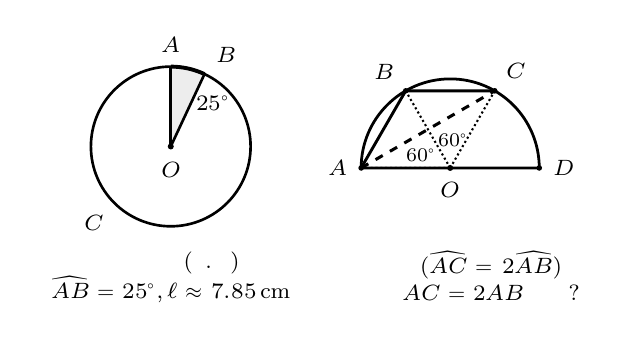
\begin{tikzpicture}[scale=0.78, every node/.style={font=\footnotesize, text=black}]
  % ឆ្វេង៖ កំណែលំហាត់ទី១ ទំ.២០៤ (<AOB = 25°, r = 18 cm)
  \begin{scope}[shift={(0,0)}]
    \coordinate (O) at (1.55,1.40);
    \fill[gray!14] (O) -- ($(O)+(65:1.30)$) arc (65:90:1.30) -- cycle;
    \draw[black, line width=0.95pt] (O) circle (1.30);
    \draw[black, line width=0.95pt] (O) -- ($(O)+(65:1.30)$);
    \draw[black, line width=0.95pt] (O) -- ($(O)+(90:1.30)$);
    \draw[black, line width=1.40pt] ($(O)+(65:1.30)$) arc (65:90:1.30);
    \fill[black] (O) circle (1.4pt) node[below=2pt] {$O$};
    \node[above=1.5pt] at ($(O)+(90:1.30)$) {$A$};
    \node[above right=1pt] at ($(O)+(65:1.30)$) {$B$};
    \node[below left=1pt] at ($(O)+(225:1.30)$) {$C$};
    \node[right=2pt] at ($(O)+(77:0.72)$) {$25^\circ$};
    \node[anchor=north, text width=3.40cm, align=center] at (1.55,-0.15) {កំណែលំហាត់ទី១ (ទំ.២០៤)៖\\$\arc{AB}=25^\circ, \ell\approx 7.85\unit{cm}$};
  \end{scope}
  % ស្ដាំ៖ បេសកកម្ម E1 ស៊ុមបង្អួចកោង (ធ្នូ 60° vs ធ្នូ 120° = 2 x 60°)
  \begin{scope}[shift={(4.50,0)}]
    \coordinate (O) at (1.60,1.05);
    \draw[black, line width=1.0pt] ($(O)+(0:1.45)$) arc (0:180:1.45) -- cycle;
    \coordinate (A) at ($(O)+(180:1.45)$);
    \coordinate (B) at ($(O)+(120:1.45)$);
    \coordinate (C) at ($(O)+(60:1.45)$);
    \coordinate (D) at ($(O)+(0:1.45)$);
    \draw[black, line width=1.05pt] (A)--(B)--(C);
    \draw[black, line width=1.10pt, dashed] (A)--(C);
    \draw[black, line width=0.75pt, densely dotted] (O)--(A) (O)--(B) (O)--(C);
    \fill[black] (O) circle (1.4pt) node[below=1.5pt] {$O$};
    \fill[black] (A) circle (1.3pt) node[left=1.5pt] {$A$};
    \fill[black] (B) circle (1.3pt) node[above left=1pt] {$B$};
    \fill[black] (C) circle (1.3pt) node[above right=1pt] {$C$};
    \fill[black] (D) circle (1.3pt) node[right=1.5pt] {$D$};
    \node at ($(O)+(156:0.52)$) {\scriptsize $60^\circ$};
    \node at ($(O)+(84:0.46)$) {\scriptsize $60^\circ$};
    \node[anchor=north, text width=3.55cm, align=center] at (1.60,-0.15) {ស៊ុមបង្អួចកោង ($\arc{AC}=2\arc{AB}$)៖\\តើអង្កត់ធ្នូ $AC = 2AB$ មែនឬទេ?};
  \end{scope}
\end{tikzpicture}}

% ២. E3 Explain: លំហាត់គំរូទី១ (អង្កត់ផ្ចិតធំជាងគេ AB > CD) និងលំហាត់គំរូទី២ (MN = PQ <=> ធ្នូ MN = ធ្នូ PQ, ទំ.២០១)
\newcommand{\figTheoremsCIRCThree}{%
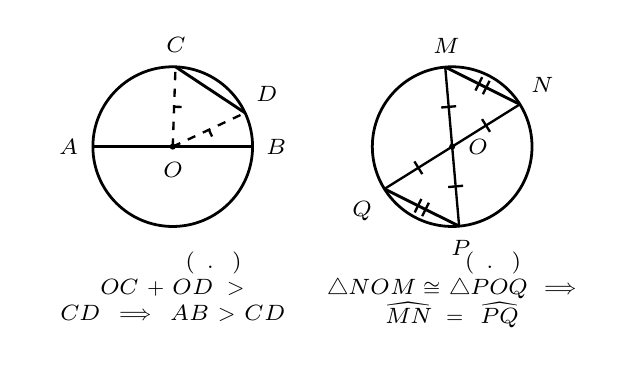
\begin{tikzpicture}[scale=0.78, every node/.style={font=\footnotesize, text=black}]
  % ឆ្វេង៖ លំហាត់គំរូទី១ ទំ.២០១ (អង្កត់ផ្ចិត AB > អង្កត់ធ្នូ CD តាមត្រីកោណ OCD)
  \begin{scope}[shift={(0,0)}]
    \coordinate (O) at (1.55,1.40);
    \draw[black, line width=1.0pt] (O) circle (1.30);
    \coordinate (A) at ($(O)+(180:1.30)$);
    \coordinate (B) at ($(O)+(0:1.30)$);
    \coordinate (C) at ($(O)+(88:1.30)$);
    \coordinate (D) at ($(O)+(25:1.30)$);
    \draw[black, line width=1.05pt] (A)--(B);
    \draw[black, line width=1.05pt] (C)--(D);
    \draw[black, line width=0.85pt, dashed, tk1] (O)--(C);
    \draw[black, line width=0.85pt, dashed, tk1] (O)--(D);
    \fill[black] (O) circle (1.4pt) node[below=2pt] {$O$};
    \node[left=1.5pt] at (A) {$A$};
    \node[right=1.5pt] at (B) {$B$};
    \node[above=1.5pt] at (C) {$C$};
    \node[above right=1pt] at (D) {$D$};
    \node[anchor=north, text width=3.45cm, align=center] at (1.55,-0.15) {លំហាត់គំរូទី១ (ទំ.២០១)៖\\$OC+OD > CD \implies AB > CD$};
  \end{scope}
  % ស្ដាំ៖ លំហាត់គំរូទី២ ទំ.២០១ (ត្រីកោណ NOM = POQ តាម ជ.ជ.ជ)
  \begin{scope}[shift={(4.50,0)}]
    \coordinate (O) at (1.60,1.40);
    \draw[black, line width=1.0pt] (O) circle (1.30);
    \coordinate (M) at ($(O)+(95:1.30)$);
    \coordinate (N) at ($(O)+(32:1.30)$);
    \coordinate (P) at ($(O)+(-85:1.30)$);
    \coordinate (Q) at ($(O)+(-148:1.30)$);
    \draw[black, line width=0.85pt, tk1] (O)--(M);
    \draw[black, line width=0.85pt, tk1] (O)--(N);
    \draw[black, line width=0.85pt, tk1] (O)--(P);
    \draw[black, line width=0.85pt, tk1] (O)--(Q);
    \draw[black, line width=1.05pt, tk2] (M)--(N);
    \draw[black, line width=1.05pt, tk2] (P)--(Q);
    \fill[black] (O) circle (1.4pt) node[right=2.5pt] {$O$};
    \node[above=1.5pt] at (M) {$M$};
    \node[above right=1pt] at (N) {$N$};
    \node[below=1.5pt] at (P) {$P$};
    \node[below left=1pt] at (Q) {$Q$};
    \node[anchor=north, text width=3.50cm, align=center] at (1.60,-0.15) {លំហាត់គំរូទី២ (ទំ.២០១)៖\\$\tri{NOM}\cg\tri{POQ} \implies \arc{MN}=\arc{PQ}$};
  \end{scope}
\end{tikzpicture}}

% ៣. E4 & E5: លំហាត់គំរូទី៣ (ទំ.២០១) + លំហាត់ទី២ និងទី៣ (ទំ.២០៤ ធ្នូត្រួតគ្នា)
\newcommand{\figOverlapChordsCIRCThree}{%
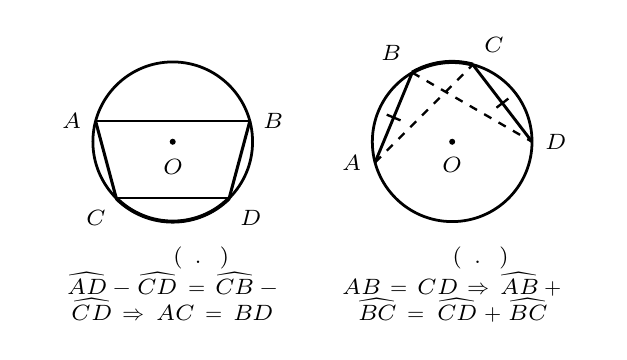
\begin{tikzpicture}[scale=0.78, every node/.style={font=\footnotesize, text=black}]
  % ឆ្វេង៖ លំហាត់ទី២ ទំ.២០៤ (ធ្នូ AD = ធ្នូ CB => ដកធ្នូរួម CD បាន AC = BD)
  \begin{scope}[shift={(0,0)}]
    \coordinate (O) at (1.55,1.40);
    \draw[black, line width=1.0pt] (O) circle (1.30);
    \coordinate (A) at ($(O)+(165:1.30)$);
    \coordinate (B) at ($(O)+(15:1.30)$);
    \coordinate (C) at ($(O)+(225:1.30)$);
    \coordinate (D) at ($(O)+(315:1.30)$);
    \draw[black, line width=0.90pt] (A)--(B) (C)--(D);
    \draw[black, line width=1.10pt] (A)--(C) (B)--(D);
    \draw[black, line width=1.40pt] (C) arc (225:315:1.30);
    \fill[black] (O) circle (1.4pt) node[below=2.5pt] {$O$};
    \node[left=1.5pt] at (A) {$A$};
    \node[right=1.5pt] at (B) {$B$};
    \node[below left=1pt] at (C) {$C$};
    \node[below right=1pt] at (D) {$D$};
    \node[anchor=north, text width=3.45cm, align=center] at (1.55,-0.15) {លំហាត់ទី២ (ទំ.២០៤)៖\\$\arc{AD}-\arc{CD}=\arc{CB}-\arc{CD} \Rightarrow AC=BD$};
  \end{scope}
  % ស្ដាំ៖ លំហាត់ទី៣ ទំ.២០៤ (AB = CD => បូកធ្នូរួម BC បាន ធ្នូ AC = ធ្នូ BD)
  \begin{scope}[shift={(4.50,0)}]
    \coordinate (O) at (1.60,1.40);
    \draw[black, line width=1.0pt] (O) circle (1.30);
    \coordinate (A) at ($(O)+(195:1.30)$);
    \coordinate (B) at ($(O)+(120:1.30)$);
    \coordinate (C) at ($(O)+(75:1.30)$);
    \coordinate (D) at ($(O)+(0:1.30)$);
    \draw[black, line width=1.05pt, tk1] (A)--(B);
    \draw[black, line width=1.05pt, tk1] (C)--(D);
    \draw[black, line width=0.85pt, dashed] (A)--(C) (B)--(D);
    \draw[black, line width=1.45pt] (C) arc (75:120:1.30);
    \fill[black] (O) circle (1.4pt) node[below=2pt] {$O$};
    \node[left=1.5pt] at (A) {$A$};
    \node[above left=1pt] at (B) {$B$};
    \node[above right=1pt] at (C) {$C$};
    \node[right=1.5pt] at (D) {$D$};
    \node[anchor=north, text width=3.50cm, align=center] at (1.60,-0.15) {លំហាត់ទី៣ (ទំ.២០៤)៖\\$AB=CD \Rightarrow \arc{AB}+\arc{BC}=\arc{CD}+\arc{BC}$};
  \end{scope}
\end{tikzpicture}}

\begin{document}
\fontsize{10pt}{15.2pt}\selectfont

% -------------------- ក្បាលកិច្ចតែងការ (Header) --------------------
\begin{center}
  {\muol\fontsize{11pt}{16pt}\selectfont ព្រះរាជាណាចក្រកម្ពុជា}\\[2pt]
  {\muol\fontsize{10pt}{15pt}\selectfont ជាតិ សាសនា ព្រះមហាក្សត្រ}\\[1pt]
  \khmflourish
\end{center}

\vspace{-28pt}
{\muol\fontsize{9.5pt}{12.5pt}\selectfont
មន្ទីរអប់រំ យុវជន និងកីឡា ខេត្តកំពង់ធំ\\
ការិយាល័យអប់រំ យុវជន និងកីឡា ស្រុកកំពង់ស្វាយ\\
អនុវិទ្យាល័យព្រះក្រសាំង}

\vspace{1pt}
\begin{center}
  {\muol\fontsize{10pt}{14pt}\selectfont កិច្ចតែងការបង្រៀន}
\end{center}
\vspace{0pt}

% -------------------- ព័ត៌មានទូទៅ (Metadata) --------------------
{\renewcommand{\arraystretch}{0.95}
\hspace*{4.05cm}%
\begin{tabular}{@{}l l l@{}}
  - \hspace{0.35cm} មុខវិជ្ជា & : & គណិតវិទ្យា ថ្នាក់ទី៨ \\
  - \hspace{0.35cm} ចំណងជើងមេរៀន & : & មេរៀនទី១៥ រង្វង់ \\
  - \hspace{0.35cm} ចំណងជើងរង & : & ២.១ ធ្នូ និងអង្កត់ធ្នូ (សៀវភៅសិក្សាគោល ទំ.២០០--២០១ និងទំ.២០៤) \\
  - \hspace{0.35cm} រយៈពេល & : & ១ ម៉ោងសិក្សា (៥០ នាទី) \\
  - \hspace{0.35cm} បង្រៀនដោយ & : & ហុក ប៊ុនថែន \\
  - \hspace{0.35cm} កាលបរិច្ឆេទ & : & ថ្ងៃសៅរ៍ ២រោច ខែមិគសិរ ព.ស.២៥៧០ (២៦ ធ្នូ ២០២៦) \\
\end{tabular}
}

\vspace{1pt}

% -------------------- I. វត្ថុបំណង --------------------
\textbf{I.} {\muol វត្ថុបំណង}\\[1pt]
\hspace*{0.55cm}%
\begin{tabular}{@{}l l L{14.2cm}@{}}
  \wcirc \hspace{0.25cm} វិជ្ជាសម្បទា & : & សិស្សពោលបានត្រឹមត្រូវនូវទ្រឹស្ដីបទទាំងបីស្ដីពីធ្នូ និងអង្កត់ធ្នូ៖ (១) អង្កត់ផ្ចិតជាអង្កត់ធ្នូធំជាងគេក្នុងរង្វង់ ($AB = 2r > CD$), (២) ធ្នូប៉ុនគ្នាសន្ធឹងដោយអង្កត់ធ្នូប៉ុនគ្នា ($\arc{AB}=\arc{MN} \implies AB=MN$), និង (៣) អង្កត់ធ្នូប៉ុនគ្នាសន្ធឹងធ្នូប៉ុនគ្នា ($AB=MN \implies \arc{AB}=\arc{MN}$) ព្រមទាំងវិសមភាពរវាងធ្នូតូច និងអង្កត់ធ្នូតាមសៀវភៅគោល ទំ.២០០--២០១ ។ \\
  \wcirc \hspace{0.25cm} បំណិនសម្បទា & : & សិស្សគូស \textbf{កាំជំនួយភ្ជាប់ផ្ចិត $O$} ដើម្បីស្រាយបញ្ជាក់ទ្រឹស្ដីបទអង្កត់ធ្នូតាមវិសមភាពត្រីកោណ និងត្រីកោណប៉ុនគ្នា (ជ.ជ.ជ) ព្រមទាំងប្រើវិធីបូក-ដកធ្នូរួមដើម្បីដោះស្រាយលំហាត់សម្រាយបញ្ជាក់លើសន្លឹកកិច្ចការស-ខ្មៅបានត្រឹមត្រូវ ។ \\
  \wcirc \hspace{0.25cm} ចរិយាសម្បទា & : & សិស្សមានទម្លាប់ផ្ទៀងផ្ទាត់អំណះអំណាងដោយវិសមភាពត្រីកោណ មិនច្រឡំសន្មតថាប្រវែងអង្កត់ធ្នូកើនឡើងសមាមាត្រត្រង់តាមដឺក្រេធ្នូ ($\arc{AC}=2\arc{AB} \not\Rightarrow AC=2AB$) និងឃើញតម្លៃអនុវត្តក្នុងសំណង់ក្លោងទ្វារ និងស៊ុមកោង ។ \\
\end{tabular}

\vspace{1pt}

% -------------------- II. សម្ភារៈឧបទេស --------------------
\textbf{II.} {\muol សម្ភារៈឧបទេស}\\[1pt]
\hspace*{0.55cm}$\bullet$ \hspace{0.35cm} សៀវភៅសិក្សាគោលគណិតវិទ្យាថ្នាក់ទី៨ (ទំ.២០០--២០១ និងទំ.២០៤) ក្ដារខៀន ដីស បន្ទាត់ក្រិត ដែកឈាន និងសន្លឹកកិច្ចការសិស្សស-ខ្មៅ (\en{Worksheet\_CIRC3} ចំនួន ២ ទំព័រ \en{A4} ដោយគ្មានស្លាយ \en{LCD}) ។

\vspace{1pt}

% -------------------- III. វិធីសាស្រ្តបង្រៀន --------------------
\textbf{III.} {\muol វិធីសាស្រ្តបង្រៀន}\\[1pt]
\hspace*{0.55cm}$\bullet$ \hspace{0.35cm} គោលវិធីសិស្សមជ្ឈមណ្ឌលតាមគំរូ \en{5Es} រួមបញ្ចូល \textbf{វិធីគូសកាំជំនួយបំប្លែងរង្វង់ជាត្រីកោណ} (\en{Auxiliary-Radii Triangle-Bridge Proof}, \en{Palatnik \& Sigler, 2019}) និង \textbf{ឧទាហរណ៍ផ្ទុយបំបែកអន្ទាក់សមាមាត្រអង្កត់ធ្នូ} (\en{De Bock et al., 2002}) ។

\vspace{2pt}

% -------------------- IV. ដំណើរការបង្រៀន --------------------
\textbf{IV.} {\muol ដំណើរការបង្រៀន}\\[-6pt]

{\renewcommand{\arraystretch}{1.15}
\begin{longtable}{|L{5.50cm}|L{7.90cm}|L{4.80cm}|}
\hline
\multicolumn{1}{|c|}{\cellcolor{headgray}\muol សកម្មភាពគ្រូ} &
\multicolumn{1}{c|}{\cellcolor{headgray}\muol ខ្លឹមសារមេរៀន} &
\multicolumn{1}{c|}{\cellcolor{headgray}\muol សកម្មភាពសិស្ស} \\[2pt]
\hline
\endfirsthead

\hline
\multicolumn{1}{|c|}{\cellcolor{headgray}\muol សកម្មភាពគ្រូ} &
\multicolumn{1}{c|}{\cellcolor{headgray}\muol ខ្លឹមសារមេរៀន} &
\multicolumn{1}{c|}{\cellcolor{headgray}\muol សកម្មភាពសិស្ស} \\[2pt]
\hline
\endhead

\hline
\endfoot

% ==================== ជំហានទី១ (2min) ====================
\stepheader{ជំហានទី១ ៖ រដ្ឋបាលថ្នាក់ (២ នាទី)}
$\bullet$ ពិនិត្យអវត្តមាន សណ្ដាប់ធ្នាប់ អនាម័យ និងការត្រៀមបន្ទាត់ក្រិត-ដែកឈាន \par\vspace{1pt}
$\bullet$ ចែកសន្លឹកកិច្ចការស-ខ្មៅ \en{Worksheet\_CIRC3} (១ សន្លឹកសងខាងក្នុងម្នាក់)
&
$\bullet$ វត្តមានសិស្ស វិន័យ និងការត្រៀមបន្ទាត់ក្រិត-ដែកឈាន \par\vspace{1pt}
$\bullet$ សន្លឹកកិច្ចការសិស្ស \en{Worksheet\_CIRC3} (មេរៀនទី១៥ ៖ ២.១ ធ្នូ និងអង្កត់ធ្នូ)
&
$\circ$ ប្រធានថ្នាក់រាយការណ៍អវត្តមាន \par\vspace{1pt}
$\circ$ ទទួលសន្លឹកកិច្ចការ សរសេរឈ្មោះ និងដាក់បន្ទាត់-ដែកឈានលើតុ \\
\hline

% ==================== ជំហានទី២ (9min) ====================
\stepheader{ជំហានទី២ ៖ កែកិច្ចការផ្ទះ រំលឹកមេរៀនចាស់ និងភ្ជាប់បញ្ហាថ្មី (៩ នាទី)}
\timenote{(កែកិច្ចការផ្ទះ $\le 3\unit{min}$)} \par
$\bullet$ ហៅសិស្ស ១ នាក់ឡើងបង្ហាញចម្លើយលំហាត់ទី១ (ទំ.២០៤) លើក្ដារខៀន
&
\textbf{កំណែកិច្ចការផ្ទះ (លំហាត់ទី១ ទំ.២០៤)៖} \par
$\bullet$ មុំផ្ចិត $\ang{AOB} = 25^\circ \Rightarrow$ រង្វាស់ដឺក្រេធ្នូតូច $\arc{AB} = \mathbf{25^\circ}$ និងធ្នូធំ $\arc{ACB} = 360^\circ - 25^\circ = \mathbf{335^\circ}$ ។ \par
$\bullet$ បើ $r = 18\unit{cm}$៖ $\ell_{\arc{AB}} = \dfrac{2\times 3.14\times 18\times 25^\circ}{360^\circ} = \mathbf{7.85\unit{cm}}$ ។
&
$\circ$ ផ្ទៀងផ្ទាត់ចម្លើយក្នុងសៀវភៅលំហាត់ និងកែលម្អកំហុសឆ្គង \\[3pt]

\timenote{(រំលឹកមេរៀនទាក់ទង $3\unit{min}$)} \par
$\bullet$ សួររំលឹក \textbf{វិសមភាពត្រីកោណ} និង \textbf{ករណីត្រីកោណប៉ុនគ្នាទី១ (ជ.ម.ជ) និងទី៣ (ជ.ជ.ជ)}
&
\textbf{រំលឹកចំណេះដឹងមូលដ្ឋានភ្ជាប់មេរៀនថ្មី៖} \par
១. \textbf{វិសមភាពត្រីកោណ៖} ក្នុង $\tri{OCD}$ ផលបូកប្រវែងជ្រុងពីរធំជាងជ្រុងទីបីជានិច្ច ($OC + OD > CD$) ។ \par
២. \textbf{ត្រីកោណប៉ុនគ្នា៖} ករណី (ជ.ម.ជ) និងករណី (ជ.ជ.ជ) នាំឱ្យមុំ និងជ្រុងត្រូវគ្នាប៉ុនគ្នា ។
&
$\circ$ ឆ្លើយរំលឹក៖ «ផលបូកជ្រុងពីរធំជាងជ្រុងទីបី និងត្រីកោណប៉ុនគ្នាតាម ជ.ម.ជ និង ជ.ជ.ជ» \\[3pt]

\fiveE{E1 - Engage} \timenote{(3 min)} \par
$\bullet$ លើកបញ្ហា \textbf{«របារឈើទ្រស៊ុមបង្អួចកោង»} លើក្ដារខៀន និងផ្នែកទី១ នៃសន្លឹកកិច្ចការ \par
\hspace*{0.3em}– សំណួរ៖ «បើធ្នូ $\arc{AC}$ ធំជាងធ្នូ $\arc{AB}$ ចំនួន $2$ ដង ($120^\circ = 2\times 60^\circ$) តើរបារត្រង់ (អង្កត់ធ្នូ) $AC$ វែងស្មើនឹង $2AB$ ដែរឬទេ?»
&
\textbf{បេសកកម្ម E1 ៖ ស៊ុមបង្អួចកោងកន្លះរង្វង់ ($r = 2\unit{m}$)} \par
ជាងឈើដំឡើងស៊ុមបង្អួចកន្លះរង្វង់អង្កត់ផ្ចិត $AD = 4\unit{m}$ ($r = 2\unit{m}$) ដោយចែកធ្នូ៖ $\arc{AB} = 60^\circ$ ($AB = 2\unit{m}$) និង $\arc{AC} = 120^\circ = 2\arc{AB}$ ។ \par
$\bullet$ \textbf{មតិទី១៖} ធ្នូកើន $2$ ដង នោះអង្កត់ធ្នូក៏កើន $2$ ដងដែរ ($AC = 2AB = 4\unit{m}$) ។ \par
$\bullet$ \textbf{មតិទី២៖} $AC > AB$ តែ $AC < 2AB$ (ព្រោះ $4\unit{m}$ ជាប្រវែងអង្កត់ផ្ចិត $AD$ ដែលវែងជាងគេ!) ។
&
$\circ$ អានបេសកកម្មលើសន្លឹកកិច្ចការ និងគូសធីកទស្សន៍ទាយមតិទី១ ឬមតិទី២ \\[3pt]

&
\cfig{\figEngageCIRCThree}
& \\[3pt]
\hline

% ==================== ជំហានទី៣ (17min) ====================
\stepheader{ជំហានទី៣ ៖ មេរៀនថ្មី — ធ្នូ និងអង្កត់ធ្នូ (១៧ នាទី)}
\fiveE{E2 - Explore} \timenote{(11 min)} \par
\ditem \textbf{សកម្មភាពទី១៖ វាស់ខ្នាតពិត $1:1$ និងស្ពានកាំជំនួយ ($5.5\unit{min}$)} \par
$\bullet$ ឱ្យដៃគូសិស្សវាស់ប្រវែងអង្កត់ធ្នូ $AB, BC, AC$ និងអង្កត់ផ្ចិត $AD$ លើរង្វង់ខ្នាតពិត $1:1$ ($r = 2.0\unit{cm}$ ក្នុងផ្នែកទី២ នៃសន្លឹកកិច្ចការ) និងប្រៀបធៀប $OC + OD$ ទៅនឹងអង្កត់ធ្នូ $CD$ ណាមួយ
&
\textbf{១. រុករកអង្កត់ធ្នូធំជាងគេ និងបំបែកអន្ទាក់សមាមាត្រខុស៖} \par
$\bullet$ វាស់លើរូបខ្នាតពិត $1:1$ ($r = 2.0\unit{cm}$)៖ \par
\hspace*{0.3em}– ធ្នូ $60^\circ$៖ $AB = BC = 2.0\unit{cm}$ ។ អង្កត់ផ្ចិត $AD = 4.0\unit{cm} = 2r$ ។ \par
\hspace*{0.3em}– ធ្នូ $120^\circ$ ($\arc{AC} = 2\arc{AB}$)៖ វាស់ឃើញ $AC \approx \mathbf{3.5\unit{cm}}$ ($2\sqrt{3}\approx 3.46\unit{cm}$) ដែល $AB < AC < 2AB$! \par
\hspace*{0.3em}– \textbf{មូលហេតុ៖} ក្នុងត្រីកោណ $\tri{ABC}$ តាមវិសមភាពត្រីកោណ $AB + BC > AC \implies 2AB > AC$ ។ \par
$\bullet$ សម្រាប់អង្កត់ធ្នូ $CD$ មិនកាត់តាម $O$៖ គូសកាំជំនួយ $OC, OD \Rightarrow$ ក្នុង $\tri{OCD}$ មាន $OC + OD > CD \implies 2r > CD \implies \mathbf{AD > CD}$ ។
&
$\circ$ ប្រើបន្ទាត់ក្រិតវាស់ឃើញ $AC \approx 3.5\unit{cm} < 4.0\unit{cm}$ បដិសេធមតិទី១ \par\vspace{1pt}
$\circ$ គូសកាំជំនួយ $OC, OD$ ទាញបានអង្កត់ផ្ចិតធំជាងអង្កត់ធ្នូទាំងអស់ \\[3pt]

\ditem \textbf{សកម្មភាពទី២៖ សមមូលរវាងធ្នូ និងអង្កត់ធ្នូតាមត្រីកោណកាំ ($5.5\unit{min}$)} \par
$\bullet$ ឱ្យសិស្សពិនិត្យត្រីកោណកាំ $\tri{OAB}$ និង $\tri{OMN}$ លើសន្លឹកកិច្ចការ៖ បើ $\arc{AB} = \arc{MN}$ តើមុំផ្ចិតស្មើគ្នាឬទេ? ចុះច្រាសមកវិញបើ $AB = MN$ តើត្រីកោណទាំងពីរប៉ុនគ្នាតាមករណីអ្វី?
&
\textbf{២. រុករកសមមូលរវាងធ្នូប៉ុនគ្នា និងអង្កត់ធ្នូប៉ុនគ្នា (ទំ.២០០--២០១)៖} \par
$\bullet$ \textbf{ទិសដៅទី១ ($\arc{AB} = \arc{MN} \implies AB = MN$)៖} \par
\hspace*{0.3em}$\arc{AB} = \arc{MN} \implies \ang{AOB} = \ang{MON}$ ។ ដោយ $OA=OB=OM=ON=r$ នោះ $\tri{AOB} \cg \tri{MON}$ តាមករណី \textbf{(ជ.ម.ជ)} $\implies AB = MN$ ។ \par
$\bullet$ \textbf{ទិសដៅច្រាស ($AB = MN \implies \arc{AB} = \arc{MN}$)៖} \par
\hspace*{0.3em}ក្នុង $\tri{AOB}$ និង $\tri{MON}$ មាន $OA=OM=r, OB=ON=r$ និង $AB=MN \implies \tri{AOB} \cg \tri{MON}$ តាមករណី \textbf{(ជ.ជ.ជ)} $\implies \ang{AOB} = \ang{MON} \implies \arc{AB} = \arc{MN}$ ។
&
$\circ$ បំពេញជំហានបង្ហាញ $\tri{AOB}\cg\tri{MON}$ ទាំងតាម (ជ.ម.ជ) និងតាម (ជ.ជ.ជ) លើសន្លឹកកិច្ចការ \\[3pt]

\fiveE{E3 - Explain} \timenote{(6 min)} \par
$\bullet$ សំយោគសញ្ញាសម្គាល់ និងទ្រឹស្ដីបទទាំង ៣ តាមសៀវភៅគោល ទំ.២០០--២០១ លើក្ដារខៀន
&
{\muol ២.១ ធ្នូ និងអង្កត់ធ្នូ — ទ្រឹស្ដីបទ (សៀវភៅគោល ទំ.២០០--២០១)} \par
$\bullet$ \textbf{កំណត់សរសេរ៖} ធ្នូ $AB$ កំណត់សរសេរ $\arc{AB}$ ឯអង្កត់ធ្នូកំណត់សរសេរ $AB$ ។ \par
$\bullet$ \textbf{ទ្រឹស្ដីបទទី១៖} \textbf{អង្កត់ផ្ចិត} ជាអង្កត់ធ្នូដែលធំជាងគេនៅក្នុងរង្វង់មួយ ($d = 2r > CD$) ។ \par
$\bullet$ \textbf{ទ្រឹស្ដីបទទី២៖} ក្នុងរង្វង់មួយ ឬរង្វង់ពីរប៉ុនគ្នា បើ \textbf{ធ្នូប៉ុនគ្នា} នោះអង្កត់ធ្នូដែលសន្ធឹងធ្នូទាំងពីរនោះក៏ប៉ុនគ្នាដែរ ($\arc{AB} = \arc{MN} \implies AB = MN$) ។ \par
$\bullet$ \textbf{ទ្រឹស្ដីបទទី៣ (ច្រាស)៖} កាលណាបើ \textbf{អង្កត់ធ្នូពីរប៉ុនគ្នា} ធ្នូដែលសន្ធឹងក្រោមអង្កត់ធ្នូទាំងពីរក៏ប៉ុនគ្នាដែរ ($AB = MN \implies \arc{AB} = \arc{MN}$) ។
&
$\circ$ បំពេញទ្រឹស្ដីបទទាំងបីក្នុងផ្នែកទី៣ នៃសន្លឹកកិច្ចការ \\[3pt]

&
\cfig{\figTheoremsCIRCThree}
& \\[3pt]

$\bullet$ បន្ថែមលក្ខណៈវិសមភាពរវាងធ្នូតូច និងអង្កត់ធ្នូ (លំហាត់គំរូទី៣ ទំ.២០១) និងធនាគារហេតុផល \cnum{1}--\cnum{5}
&
{\fontsize{9.2pt}{13pt}\selectfont
\begin{tabular}[t]{|L{7.55cm}|}
\hline
\cellcolor{headgray}\textbf{ធនាគារហេតុផល (\en{Warrant Bank}) សម្រាប់ធ្នូ និងអង្កត់ធ្នូ} \\[2pt]
\hline
\cnum{1} ទ្រឹស្ដីបទអង្កត់ផ្ចិត៖ អង្កត់ផ្ចិតជាអង្កត់ធ្នូធំជាងគេក្នុងរង្វង់ ($AB = 2r \ge CD$) \par
\cnum{2} ទ្រឹស្ដីបទធ្នូស្មើគ្នា៖ $\arc{AB} = \arc{MN} \implies AB = MN$ (តាម $\tri{OAB}\cg\tri{OMN}$ ជ.ម.ជ) \par
\cnum{3} ទ្រឹស្ដីបទច្រាសអង្កត់ធ្នូស្មើគ្នា៖ $AB = MN \implies \arc{AB} = \arc{MN}$ (តាម $\tri{OAB}\cg\tri{OMN}$ ជ.ជ.ជ) \par
\cnum{4} វិសមភាពធ្នូតូច និងអង្កត់ធ្នូ ($\arc{AB} < 180^\circ$)៖ $\arc{AB} > \arc{CD} \iff \ang{AOB} > \ang{COD} \iff AB > CD$ \par
\cnum{5} ប្រមាណវិធីបូក-ដកធ្នូរួម៖ បើ $\arc{AD} = \arc{CB}$ នោះ $\arc{AD} \pm \arc{CD} = \arc{CB} \pm \arc{CD}$ \\[2pt]
\hline
\end{tabular}}\par\vspace{2pt}
&
$\circ$ ផ្ទៀងផ្ទាត់លេខកូដហេតុផល \cnum{1}--\cnum{5} លើសន្លឹកកិច្ចការ \\
\hline

% ==================== ជំហានទី៤ (20min) ====================
\stepheader{ជំហានទី៤ ៖ ពង្រឹងចំណេះដឹង និងវាយតម្លៃ (២០ នាទី)}
\fiveE{E4 - Elaborate} \timenote{(10 min)} \par
\ditem \textbf{គំរូទី១៖ លំហាត់គំរូទី១ និងទី៣ សៀវភៅគោល ទំ.២០១ ($5\unit{min}$)} \par
$\bullet$ ដឹកនាំសិស្សបំពេញសម្រាយបញ្ជាក់ $AB > CD$ (ពេល $AB$ ជាអង្កត់ផ្ចិត និងពេល $\arc{AB} > \arc{CD}$ ជាធ្នូតូច) ក្នុងផ្នែកទី៤ នៃសន្លឹកកិច្ចការ
&
\textbf{គំរូទី១ (លំហាត់គំរូទី១ និងទី៣ ទំ.២០១ — វិសមភាពអង្កត់ធ្នូ)៖} \par
$\bullet$ \textbf{ករណី $AB$ ជាអង្កត់ផ្ចិត៖} ភ្ជាប់កាំ $OC, OD$ ។ ក្នុង $\tri{CDO}$ មាន $OC + OD > CD$ $(i)$ តែ $OC + OD = r + r = AB$ $(ii) \implies \mathbf{AB > CD}$ (តាម \cnum{1}) ។ \par
$\bullet$ \textbf{ករណីធ្នូតូច $\arc{AB} > \arc{CD}$៖} ក្នុង $\tri{AOB}$ និង $\tri{COD}$ មាន $OA=OB=OC=OD=r$ ហើយដោយ $\arc{AB} > \arc{CD} \implies \ang{AOB} > \ang{COD} \implies$ ជ្រុងឈម $\mathbf{AB > CD}$ (តាម \cnum{4}) ។
&
$\circ$ បំពេញជំហានកាំជំនួយ $OC, OD$ និងសន្និដ្ឋានតាម \cnum{1}, \cnum{4} លើសន្លឹកកិច្ចការ \\[3pt]

\ditem \textbf{គំរូទី២៖ លំហាត់ទី២ សៀវភៅគោល ទំ.២០៤ — ដកធ្នូរួម ($5\unit{min}$)} \par
$\bullet$ ណែនាំយុទ្ធវិធីសម្គាល់ធ្នូរួម $\arc{CD}$ លើរូប (ដៅធ្នូដិតស-ខ្មៅ) រួចដកធ្នូរួមចេញពីអង្គទាំងពីរ
&
\textbf{គំរូទី២ (លំហាត់ទី២ ទំ.២០៤ — ស្រាយថា $AC = BD$)៖} \par
ក្នុងរង្វង់ $C(O,r)$ ចំណុច $A, C, D, B$ ស្ថិតតាមលំដាប់លើរង្វង់ ដែល $\arc{AD} = \arc{CB}$ ។ ស្រាយបញ្ជាក់ថាអង្កត់ធ្នូ $AC = BD$ ។ \par
$\bullet$ បំបែកធ្នូតាមចំណុចកណ្ដាល៖ $\arc{AD} = \arc{AC} + \arc{CD}$ និង $\arc{CB} = \arc{CD} + \arc{DB}$ ។ \par
$\bullet$ ដកធ្នូរួម $\arc{CD}$ ពីអង្គទាំងពីរនៃ $\arc{AD} = \arc{CB}$ (តាម \cnum{5})៖ \par
\hspace*{0.3em}$\arc{AD} - \arc{CD} = \arc{CB} - \arc{CD} \implies \arc{AC} = \arc{DB}$ ។ \par
$\bullet$ តាមទ្រឹស្ដីបទធ្នូប៉ុនគ្នា (\cnum{2})៖ $\arc{AC} = \arc{DB} \implies \mathbf{AC = BD}$ ។
&
$\circ$ គូសសម្គាល់ធ្នូរួម $\arc{CD}$ បំពេញការដកធ្នូរួម និងទាញបាន $AC = BD$ តាម \cnum{2} \\[3pt]

&
\cfig{\figOverlapChordsCIRCThree}
& \\[3pt]

$\bullet$ \textbf{សំណួរឆ្លុះបញ្ចាំង (\en{EIA Looking-Back})៖} \par
\hspace*{0.3em}– សួរ៖ «ហេតុអ្វីបានជាការគូស \textbf{កាំជំនួយពីផ្ចិត $O$} ជាគន្លឹះទី១ ស្ទើរគ្រប់លំហាត់សម្រាយបញ្ជាក់ក្នុងរង្វង់?»
&
$\bullet$ \textbf{គន្លឹះឆ្លុះបញ្ចាំងវិធីស្រាយបញ្ជាក់ (\en{Looking-Back})៖} \par
\hspace*{0.3em}– កាំទាំងអស់នៃរង្វង់តែមួយមានប្រវែងស្មើគ្នាជានិច្ច ($OA=OB=OC=OD=r$) ដូច្នេះការភ្ជាប់ផ្ចិត $O$ ទៅចុងអង្កត់ធ្នូបង្កើតបាន \textbf{ត្រីកោណសមបាទ} ភ្លាមៗ ដែលអនុញ្ញាតឱ្យប្រើត្រីកោណប៉ុនគ្នា និងវិសមភាពត្រីកោណបានយ៉ាងងាយ ។
&
$\circ$ ឆ្លើយសង្ខេប៖ «ព្រោះកាំទាំងអស់ស្មើនឹង $r$ បង្កើតបានជ្រុងស្មើគ្នាសម្រាប់ត្រីកោណប៉ុនគ្នា» \\[3pt]

\fiveE{E5 - Evaluate} \timenote{(10 min)} \par
\ditem \textbf{អនុវត្តផ្ទាល់ — លំហាត់ទី៣ សៀវភៅគោល ទំ.២០៤ ($6.5\unit{min}$)៖} \par
$\bullet$ ឱ្យសិស្សធ្វើលំហាត់ទី៣ (ទំ.២០៤៖ $AB = CD \implies \arc{AC} = \arc{BD}$) និងគណនាប្រវែងអង្កត់ធ្នូអតិបរមា ក្នុងផ្នែកទី៥ នៃសន្លឹកកិច្ចការ រួចប្ដូរផ្ទៀងជាដៃគូ
&
\textbf{១. អនុវត្តលំហាត់ទី៣ (ទំ.២០៤)៖} ក្នុងរង្វង់ផ្ចិត $O$ អង្កត់ធ្នូ $AB = CD$ (ចំណុច $A, B, C, D$ តាមលំដាប់លើរង្វង់) ។ ស្រាយបញ្ជាក់ថា $\arc{AC} = \arc{BD}$ ។ \par
$\bullet$ ដោយអង្កត់ធ្នូ $AB = CD \implies \arc{AB} = \arc{CD}$ (តាម \cnum{3}) ។ \par
$\bullet$ បូកធ្នូរួម $\arc{BC}$ ទៅនឹងអង្គទាំងពីរ (តាម \cnum{5})៖ \par
\hspace*{0.3em}$\arc{AB} + \arc{BC} = \arc{CD} + \arc{BC} \implies \boxed{\arc{AC} = \arc{BD}}$ ។ \par
\textbf{២. ពិនិត្យលក្ខខណ្ឌអង្កត់ធ្នូធំបំផុត៖} រង្វង់ $C(O, 6.5\unit{cm})$ មានអង្កត់ធ្នូវែងបំផុតស្មើនឹងអង្កត់ផ្ចិត $d = 2r = 2(6.5) = \mathbf{13\unit{cm}}$ ($\Rightarrow$ មិនអាចមានអង្កត់ធ្នូប្រវែង $14\unit{cm}$ ទេ!) ។
&
$\circ$ សរសេរសម្រាយបញ្ជាក់បូកធ្នូរួម $\arc{BC}$ និងគណនាអង្កត់ធ្នូអតិបរមា $13\unit{cm}$ រួចផ្ទៀងជាដៃគូ \\[3pt]

\ditem \textbf{បិទបេសកកម្ម E1 និងតេស្តរហ័ស \en{Exit Check} ($3.5\unit{min}$)៖} \par
$\bullet$ សួរបិទបេសកកម្មស៊ុមបង្អួចកោង និងឱ្យសិស្សជ្រើសរើស \en{A--D}
&
$\bullet$ \textbf{បិទបេសកកម្ម E1៖} \textbf{មតិទី២ ត្រឹមត្រូវ} — ពេលធ្នូកើន $2$ ដង ($60^\circ \to 120^\circ$) អង្កត់ធ្នូ $AC \approx 3.46\unit{m}$ ធំជាង $AB = 2\unit{m}$ តែតូចជាង $2AB = 4\unit{m}$ ជានិច្ច ។ \par
$\bullet$ \textbf{Exit Check៖} ក្នុងរង្វង់ $C(O, 5\unit{cm})$ គេមានធ្នូតូច $\arc{MN} = 70^\circ$ និង $\arc{PQ} = 140^\circ$ ។ តើទំនាក់ទំនងណាត្រឹមត្រូវ? \par
\en{A.} $PQ = 2MN$ \quad \en{B.} $PQ = MN$ \quad \graybox{\enbf{C.} $MN < PQ < 10\unit{cm}$ និង $PQ < 2MN$ \ding{51}} \quad \en{D.} $PQ = 12\unit{cm}$
&
$\circ$ លើកម្រាមដៃទី៣ ជ្រើសរើស \textbf{C} តាម \cnum{1}, \cnum{4} និងវិសមភាពត្រីកោណ \\
\hline

% ==================== ជំហានទី៥ (<=2min) ====================
\stepheader{ជំហានទី៥ ៖ កិច្ចការផ្ទះ និងបណ្ដាំផ្ញើ ($\le$ ២ នាទី)}
$\bullet$ កត់ត្រាកិច្ចការផ្ទះលើក្ដារខៀន (មានបោះពុម្ពស្រាប់នៅផ្នែកទី៦ នៃសន្លឹកកិច្ចការទំព័រទី២)
&
\textbf{កិច្ចការផ្ទះ (សៀវភៅសិក្សាគោល ទំ.២០១ និងទំ.២០៤)៖} \par
១. \textbf{លំហាត់ទី៥ (ទំ.២០៤)៖} គេឱ្យរង្វង់ $C(O, r)$ ដែលអង្កត់ធ្នូ $AB = CD$ (ចំណុច $A, C, B, D$ ស្ថិតតាមលំដាប់លើរង្វង់) ។ បង្ហាញថាធ្នូ $\arc{BD} = \arc{AC}$ ។ \par
២. \textbf{លំហាត់គំរូទី២ (ទំ.២០១ — សរសេរឡើងវិញដោយខ្លួនឯង)៖} ក្នុងរង្វង់ផ្ចិត $O$ បើ $\arc{MN} = \arc{PQ}$ ចូរស្រាយបញ្ជាក់ថាអង្កត់ធ្នូ $MN = PQ$ តាមត្រីកោណប៉ុនគ្នា ។
&
$\circ$ កត់ត្រាកិច្ចការផ្ទះ និងទុកដាក់សន្លឹកកិច្ចការក្នុងសៀវភៅសរសេរ \\[3pt]

$\bullet$ ណែនាំឱ្យអានចំណុចបញ្ចប់នៃមេរៀនទី១៥ ជាមុន
&
$\bullet$ \textbf{អានជាមុន៖} ចំណុច \textbf{២.២ លក្ខណៈឆ្លុះនៃរង្វង់} (ទំព័រ ២០២--២០៣) ។ \par
$\bullet$ \textbf{បណ្ដាំផ្ញើ៖} ត្រៀមបន្ទាត់ក្រិត ដែកឈាន និងអេគែរ (បន្ទាត់កែង) សម្រាប់សិក្សាអង្កត់ផ្ចិតកែងនឹងអង្កត់ធ្នូនៅម៉ោងក្រោយ ។
&
$\circ$ ទទួលបណ្ដាំផ្ញើ និងជម្រាបលាគ្រូ \\

\end{longtable}
}

\vspace{8pt}

% -------------------- ហត្ថលេខា (Signature Block) --------------------
\begin{flushright}
\begin{minipage}{9.6cm}
\centering
ថ្ងៃសៅរ៍ ២រោច ខែមិគសិរ ឆ្នាំមមី អដ្ឋស័ក ពុទ្ធសករាជ ២៥៧០\\[2pt]
ព្រះក្រសាំង, ថ្ងៃទី២៦ ខែធ្នូ ឆ្នាំ២០២៦\\[4pt]
{\muol គ្រូបង្រៀន}\\[32pt]
\hfill{\muol ហុក ប៊ុនថែន}\hspace*{1.4cm}
\end{minipage}
\end{flushright}

\end{document}
